\documentclass[a4paper, 12pt]{article}
\usepackage{titling}
\usepackage[margin=3.0cm]{geometry}
\usepackage{graphicx}
\usepackage{amsmath}
\usepackage{amssymb}
\usepackage{lipsum}
\usepackage{hyperref}
\usepackage[style=ieee, url=false, doi=false, isbn=false]{biblatex}
\addbibresource{bibliography.bib}

\begin{document}

\title{\bf Random Features and the Jamming Transition in Artificial Neural Networks}
\author{
    Hudson Cooper\\ % REDACT FOR SUBMISSION
    King's College London\\
    M.Sc.\ in Complex Systems Modelling
}
\date{\today}

\begin{titlingpage}
\maketitle
\begin{abstract}
\lipsum[1]
\end{abstract}
\end{titlingpage}

\section{Introduction}
Neural networks are one of the most highly successful classes of models in modern machine learning. While there is a rich body of literature which empirically examines the ability of neural networks to fit to and generalize from data, the field is lacking a cohesive theoretical framework for designing these networks and for understanding their incredible success. \\

\subsection{Motivation}

Until recently, one of the most poorly understood features of modern neural networks is their operation in a regime that is seemingly at odds with the bias-variance trade-off, a main tenet of classical statistical learning. The bias-variance trade-off implies that more expressive models are likely to find spurious patterns in data, and therefore practitioners should seek to build models that are ``as simple as possible, but no simpler." Neural networks, however, typically operate in an extremely over-parameterized regime, containing many more parameters than there are data. Neural networks have been shown to be so highly expressive that they are able to interpolate data and perfectly classify training data, even when labels have been replaced with pure noise \cite{zhangUnderstandingDeepLearning2017}. Despite their complexity and extreme expressiveness, they are able to generalize extremely well in practice, often outperforming classical models on test data. \\

Recent work \cite{belkinReconcilingModernMachine2019} has characterised this phenomena in terms of the so-called ``double-descent" curve, which is visually represented in figure \ref{doubledescent}. Two distinct regimes of model complexity are separated by the interpolation threshold, the point at which models are able to obtain perfect performance on training data at the cost of extremely high test error. To the left of this threshold is the under-parameterized regime, in which the classical bias-variance trade-off holds. As model complexity increases, generalization error follows a U-shaped curve, decreasing to a minimum before increasing to a peak, sometimes referred to as the ``generalization cusp," at the interpolation threshold, the neighborhood in which classical ``overfitting" occurs. To the right of this threshold, however, the generalization error again decreases, whith the global optimum being found deep in the over-parameterized regime or even in the limit of ``infinite" complexity. This double-descent phenomenology is far from unique to neural networks and has been observed in a variety of other estimators that are expressive enough to perfectly interpolate the training data, including random forests, random feature models, and kernel machines \cite{ belkinReconcilingModernMachine2019, belkinUnderstandDeepLearning2018}.\\

\begin{figure}[ht]
\centering
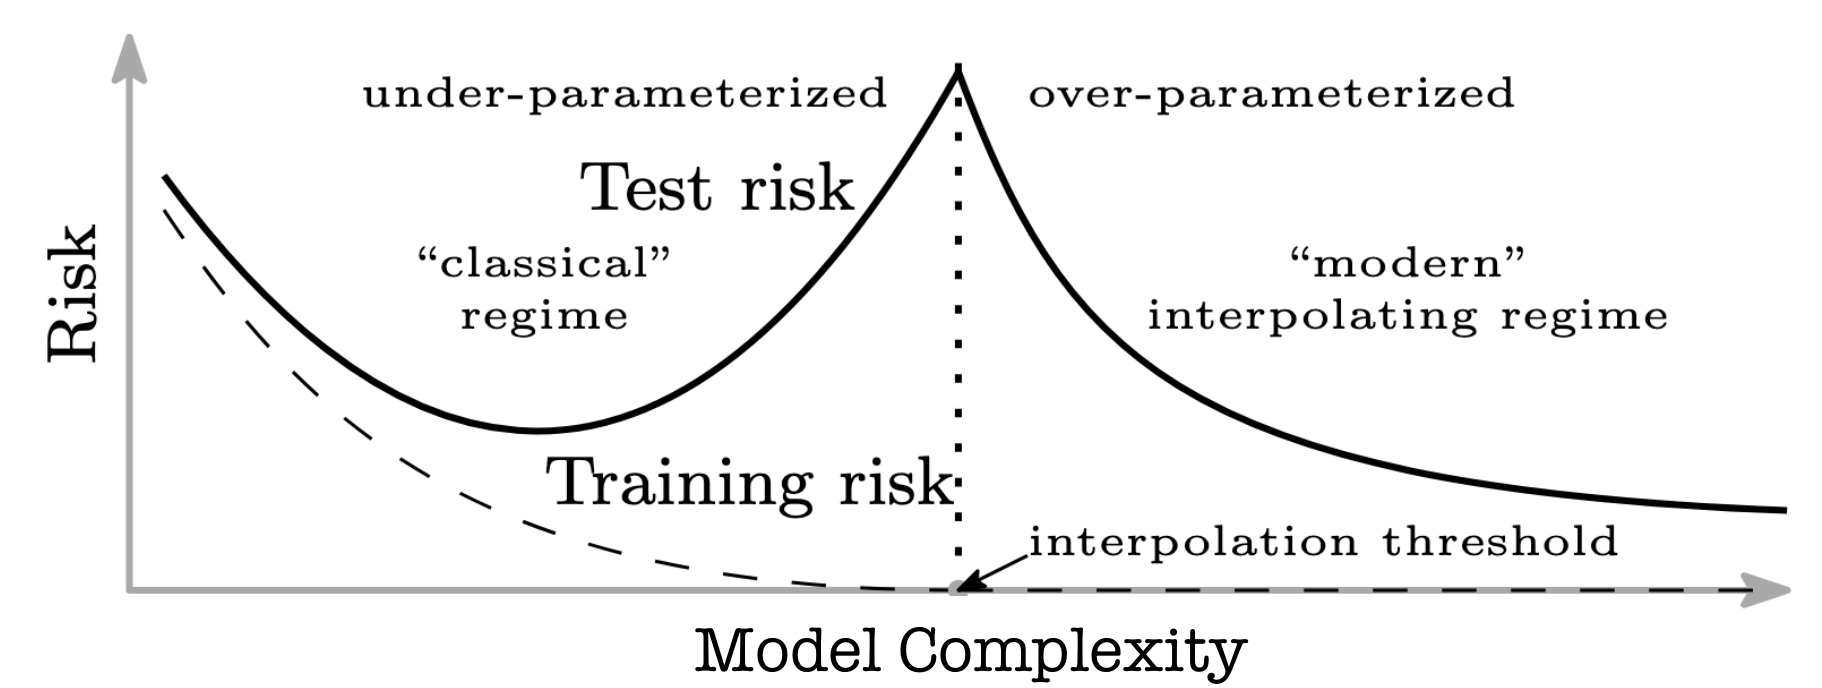
\includegraphics[width=0.7\textwidth]{docs/assets/double_descent_reconciling.png}
\caption{Visual depiction of the double descent curve, adapted from \cite{belkinReconcilingModernMachine2019}. The ``classical" U-shaped bias-variance trade-off is seen in the under-parameterized regime to the left of the interpolation threshold, and a second descent is seen in the over-parameterized regime to the right. Training error (``risk'') is represented with a dashed line, and test error is represented with a solid line.}
\label{doubledescent}
\end{figure}


Study of the training dynamics of neural networks undergoing stochastic gradient descent (SGD)  has revealed deep qualitative similarities between the interpolation threshold and the ``jamming" phase transition in granular solids \cite{baity-jesiComparingDynamicsDeep2019, geigerJammingTransitionParadigm2019}. By appealing to analogies between the physical phenomena of jamming and the separation of the under- and over-parameterized regimes by the interpolation threshold in neural networks, \cite{geigerJammingTransitionParadigm2019} and \cite{spiglerJammingTransitionOverparametrization2019} predict and empirically test a characterization of the training dynamics near and beyond the threshold. 
\\
TODO: More here. What are the analogies? 
\\

It is no surprise that over-parameterized neural networks are expressive enough achieve arbitrarily small training loss; however, it is highly non-trivial that they are able to do so without getting stuck in local minima since their loss landscapes are generally non-convex and non-smooth loss landscapes. Strong analogies between neural networks and statistical-physics models of systems with many interacting components, in particular mean-field spin-glass models, suggest that networks trained with stochastic gradient descent (SGD) from random initialization should converge to high and wide local minima despite the existence of deeper local and global minima \cite{choromanskaLossSurfacesMultilayer}. In practice, however, SGD almost never encounters any such obstacles, and global minima are easily found \cite{goodfellowQualitativelyCharacterizingNeural2015}.

\subsection{Goals and Roadmap}

The goal of this paper is to examine a recently popular model for understanding neural networks, the "random features" model. The random features model displays the characteristics of double descent independently of the training dynamics used. We therefore explore whether the jamming phenomenology is recovered by the random features model and the extent to which feature learning plays a role in its emergence.\\


This paper will conduct a review of... and then explain the novel contributions, then... OUTLINE GOES HERE

\section{Background}
\subsection{The Neural Tangent Kernel and ``Lazy Learning"}

By taking the limit as network width goes to infinity, an important connection between wide neural networks and kernel methods has been uncovered. In particular, \cite{jacotNeuralTangentKernel2018} showed that gradient-descent on network parameters corresponds to kernel gradient-descent on network outputs with respect to the so-called ``Neural Tangent Kernel" (NTK). In the infinite width limit, the NTK converges to a deterministic limiting kernel that depends only on the network architecture, is independent of parameter initialization, and is constant throughout training. This limit is referred to as the ``lazy learning" limit because the NTK does not depend on the data-set. Although the derivation is exact only in the infinite-width limit, experimental evidence in \cite{jacotNeuralTangentKernel2018} shows good agreement between both the training dynamics and final predictions of the limiting NTK machine and networks trained in the large but finite width setting under a variety of conditions, including practical architectures. Further work in \cite{allen-zhuConvergenceTheoryDeep2019} proved that the training dynamics of finite but overparameterized networks rapidly converge to those of the corresponding limiting NTK.\\

In the the lazy learning limit, network outputs can be expressed as a first-order Taylor expansion of the network about its initial weights at any time during training \cite{leeWideNeuralNetworks2019}. For a network $f_\theta$ with initial parameters $\theta_0$ and an initialization such that $f_{\theta_0} \approx 0$\footnote{Alternatively, one can define the network output to be $f_{\theta}(x) - f_{\theta_0}(x)$ as is seen in \cite{chizatLazyTrainingDifferentiable2020}}, we have that
\begin{equation}
    f_\theta(x) \approx \nabla_\theta \left.f_\theta(x)\right|_{\theta=\theta_0} \cdot (\theta - \theta_0)\,.
\end{equation}
In other words, networks in the lazy-learning regime are linear models of random features given by the gradient of the network with respect to its parameters at initialization. The inner product in this random feature space converges to the limiting NTK as the number of parameters goes to infinity, suggesting that finite-width networks can be conceptualized as finite-rank approximations to the limiting kernel machine, connecting finite-width networks to the random features (RF) models studied in \cite{rahimiRandomFeaturesLargeScale2008,meiGeneralizationErrorRandom2019}.

\subsection{Theoretical Victories of Lazy Learning}

The lazy-learning regime offers a greatly simplified point of view from which to understand the training dynamics and convergence properties of overparameterized neural networks. The authors of \cite{allen-zhuConvergenceTheoryDeep2019} offer a convincing explanation of the mechanisms by which overparameterized neural networks are able to avoid spurious local minima. They show that networks in the lazy regime have ``nearly-convex" loss in a sufficiently large neighborhood around initialization, allowing convergence to the global minimum in polynomial (in the number of parameters) time, rather than the exponential time expected from the analogies between neural networks and spin-glass models.\\

Due to lazy learning's connection to random-features models, it has also opened the door to understanding the generalization capabilities of networks in the overparameterized regime. RF models, as introduced in \cite{rahimiRandomFeaturesLargeScale2008}, are linear functions of random, nonlinear transformations of input data. They can be conceptualized as two-layer neural networks in which the first-layer weights (with width equal to the number of random features) are fixed at their independently random initialized values and the second layer weights are optimized freely. Note that for networks with a single hidden layer, the NTK can be exactly described by this formulation, but deeper networks require the introduction non-independently distributed first-layer weights \cite{chizatLazyTrainingDifferentiable2020}. \\

For regression on random input data with linear or Gaussian-process target functions (classification is similarly examined in \cite{dengModelDoubleDescent2020}), the authors of \cite{meiGeneralizationErrorRandom2019} develop precise asymptotic predictions for the generalization error of a RF model as the number of parameters $N$, the number of data $P$, and the input dimensionality $d$ are sent to infinity with their ratios fixed. Remarkably, they are able to recover the full double-descent phenomenology in this simplified setting, including the features that the test error diverges at the interpolation threshold, as is predicted in \cite{geigerScalingDescriptionGeneralization2019}, and that the global minimum of test error occurs in the infinitely over-parameterized regime, i.e. $N/P\rightarrow\infty$, as is predicted in \cite{belkinReconcilingModernMachine2019,belkinUnderstandDeepLearning2018} for kernel machines.\\



Building on the work of \cite{meiGeneralizationErrorRandom2019} and \cite{ geigerScalingDescriptionGeneralization2019}, which explores the role of initialization variance of the finite-rank NTK on generalization error, \cite{dascoliDoubleTroubleDouble2020} offers  ``modern" treatment of the bias-variance relationship beyond the interpolation threshold

\subsection{Feature Learning}

Despite its success in explaining some of the crucial features of training and generalization in neural networks, the lazy learning perspective misses an important aspect of modern neural networks and deep learning: the role of ``feature learning."  The authors of \cite{chizatLazyTrainingDifferentiable2020} argue that the lazy-learning phenomenon occurs due to an implicitly chosen factor which controls how model parameters scale at initialization against network width. By making this scaling factor explicit, it is possible to force a network to train either in the lazy-learning regime or in the ``feature-learning" regime, in which the NTK evolves throughout training and depends on the data-set. The feature-learning regime is also referred to as the ``mean-field" limit and is explored in some previous works, e.g. \cite{meiMeanFieldView2018}. While the dynamics of lazy learning can be described by a linear ordinary differential equation (ODE) of the network outputs and the constant NTK, the dynamics of feature-learning must be described by a more complex partial differential equation (PDE) which also depends on the distribution of the activations of the hidden neurons.\\

 While \cite{allen-zhuConvergenceTheoryDeep2019} gives guarantees on the convergence of lazy-trained networks, it is not immediately obvious that this regime is in face desirable. In particular, the role of feature learning in the ability of a neural network to generalize to unseen data is still poorly understood. Convolutional neural networks trained in the feature-learning regime have been found to outperform those trained in the lazy-learning regime, suggesting that lazy-learning does not account for the incredible success of these networks \cite{chizatLazyTrainingDifferentiable2020}. A comparison of the performance differences between lazy-learning and feature-learning across various architectures and data-sets found this out-performance to be far from universal, finding that fully-connected networks (FCNs), conversely to CNNs, work best in the lazy regime. These findings suggest that network architecture and the structure of the data play an important role in determining which regime is better \cite{geigerDisentanglingFeatureLazy2020}. The mechanisms at play, including the role of network depth and other architectural choices on the quality of the features learned, the effects of feature learning on the location of the interpolation threshold, and the effects of feature learning on convergence of the training loss, are poorly understood and remain important open questions in modern machine learning.











\subsection{The Jamming Transition: Loss Landscape and Generalization}

A related and similarly poorly-understood feature of modern neural networks is what the necessary and sufficient conditions are for them to be able to achieve arbitrarily low training error. 

Because loss functions are generally not convex, it is not obvious what the necessary conditions are to guarantee that gradient descent can fit well to the training data. 


Jamming as a paradigm..?

\section{Methods and Results}
\subsection{The Model}
\subsection{Feature Learning Near the Generalization Cusp}
\subsection{The Effects of Regularization}

\section{Discussion}

Still poorly understood:\\
- why, when, and how feature learning improves generalization\\
- how the location of the interpolation threshold is affected by feature learning\\
- how the ability of a network to build quality features depends on architecture (and relationship to inductive bias) \\
- double descent: a property of dynamics or a property of features?\\
- the role that feature learning plays in the emergence of the jamming phenomenology\\

\printbibliography
\end{document}